\documentclass[a4paper,12pt,twoside]{memoir}
\usepackage{btp} % Use the trainermanual package option (i.e. \usepackage[trainermanual]{btp}) to generate the Trainer's version of the manual

% Set some Workshop specific info
\setWorkshopTitle{Introduction to RNA-Seq Hands-on Workshop}
\setWorkshopVenue{Adelaide, Australia}
\setWorkshopDate{18th Apr. 2013}
\setWorkshopAuthor{
Nathan S. Watson-Haigh (ACPFG)\\
Ute Baumann (ACPFG)\\
Rad Suchecki (ACPFG)\\
John Toubia (ACPFG)\\
Timo Tiirikka (ACPFG)\\
Bastien Llamas (ACAD)\\
David Lawrence (ACRF Cancer Genomics Facility)\\
Katherine Pillman (CCB)\\
}

\begin{document}

%
% Workshop Title Page
%
\workshoptitlepage

%
% CC-BY
%
\chapter{Licensing}

This work is licensed under a Creative Commons Attribution 3.0 Unported License and
the below text is a summary of the main terms of the full Legal Code (the full licence) available at
\url{http://creativecommons.org/licenses/by/3.0/legalcode}.

\begin{description}[style=multiline,labelindent=0cm,align=left,leftmargin=1.5cm]
\item[You are free:] \hfill

to copy, distribute, display, and perform the work 

to make derivative works

to make commercial use of the work
  
\item[Under the following conditions:] \hfill

  \textbf{Attribution} - You must give the original author credit.
  
\item[With the understanding that:] \hfill

  \textbf{Waiver} - Any of the above conditions can be waived if you get permission from the
  copyright holder.
  
  \textbf{Public Domain} - Where the work or any of its elements is in the public domain
  under applicable law, that status is in no way affected by the license.
  
  \textbf{Other Rights} - In no way are any of the following rights affected by the license:
  
  \begin{itemize}
    \item Your fair dealing or fair use rights, or other applicable copyright exceptions and limitations;
  
    \item The author's moral rights;
  
    \item Rights other persons may have either in the work itself or in how the work is used, such
    as publicity or privacy rights.
  \end{itemize}
  
  \textbf{Notice} - For any reuse or distribution, you must make clear to others the
  licence terms of this work.
  
\end{description}

\vspace{\fill}

\begin{center}

\includegraphics[height=1cm]{./licences/cc_by.png}
\end{center}

\clearpage

\tableofcontents

\chapter{Workshop Information}
\clearpage

%
% Trainers Page
%
\section{The Trainers}

\newlength{\trainerIconWidth}
\setlength{\trainerIconWidth}{2.0cm}

\begin{table}[H]
  \centering
  \small
  \renewcommand{\arraystretch}{1}
  %\caption{A table arranging  images}
  \rowcolors{1}{gray!25}{white}
  \begin{tabular}{>{\centering\arraybackslash} m{1.1\trainerIconWidth} m{1\textwidth}}
    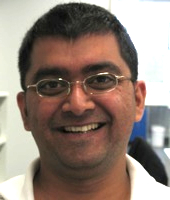
\includegraphics[width=\trainerIconWidth]{graphics/Deshpande.jpg} & 
      \textbf{Dr. Nandan Deshpande}\newline
      
      Postdoctoral Fellow\newline
      The University of New South Wales (UNSW), NSW\newline
      \mailto{n.deshpande@unsw.edu.au}\\
    
    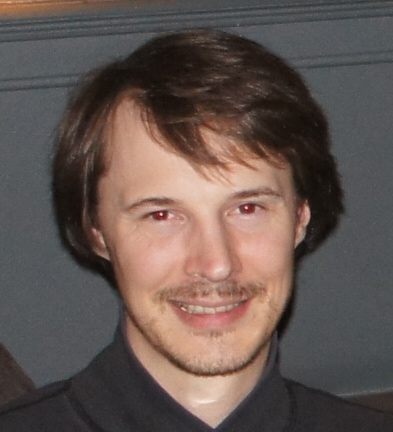
\includegraphics[width=\trainerIconWidth]{graphics/Duesing.jpg} & 
      \textbf{Dr. Konsta Duesing}\newline
      
      Research Team Leader - Statistics \& Bioinformatics\newline
      CSIRO Animal, Food and Health Science, NSW\newline
      \mailto{konsta.duesing@csiro.au}\\
    
    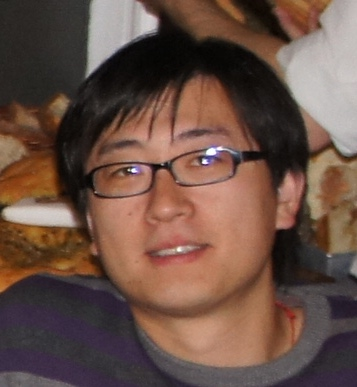
\includegraphics[width=\trainerIconWidth]{graphics/Li.jpg} & 
      \textbf{Dr. Xi (Sean) Li}\newline
      
      Bioinformatics Analyst\newline
      Bioinformatics Core, CSIRO Mathematics, Informatics and Statistics, ACT\newline
      \mailto{sean.li@csiro.au}\\
    
    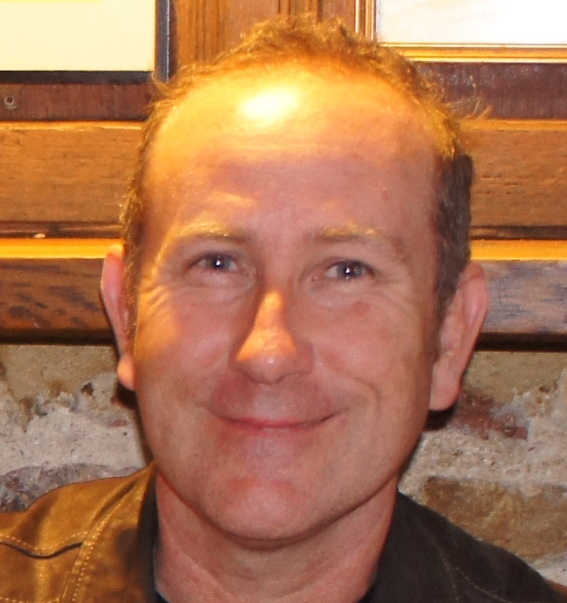
\includegraphics[width=\trainerIconWidth]{graphics/McWilliam.jpg} & 
      \textbf{Mr. Sean McWilliam}\newline
      
      Bioinformatics Analyst\newline
      CSIRO Animal, Food and Health Sciences, QLD\newline
      \mailto{sean.mcwilliam@csiro.au}\\
    
    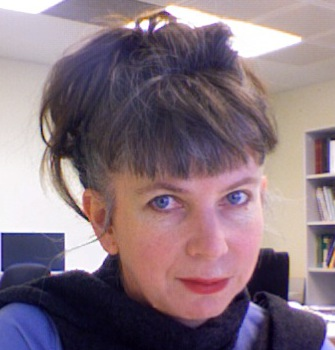
\includegraphics[width=\trainerIconWidth]{graphics/Moolhuijzen.jpg} & 
      \textbf{Dr. Paula Moolhuijzen}\newline
      
      Senior Bioinformatics Officer\newline
      Centre for Comparative Genomics, Murdoch University, WA\newline
      \mailto{pmoolhuijzen@ccg.murdoch.edu.au}\\
    
    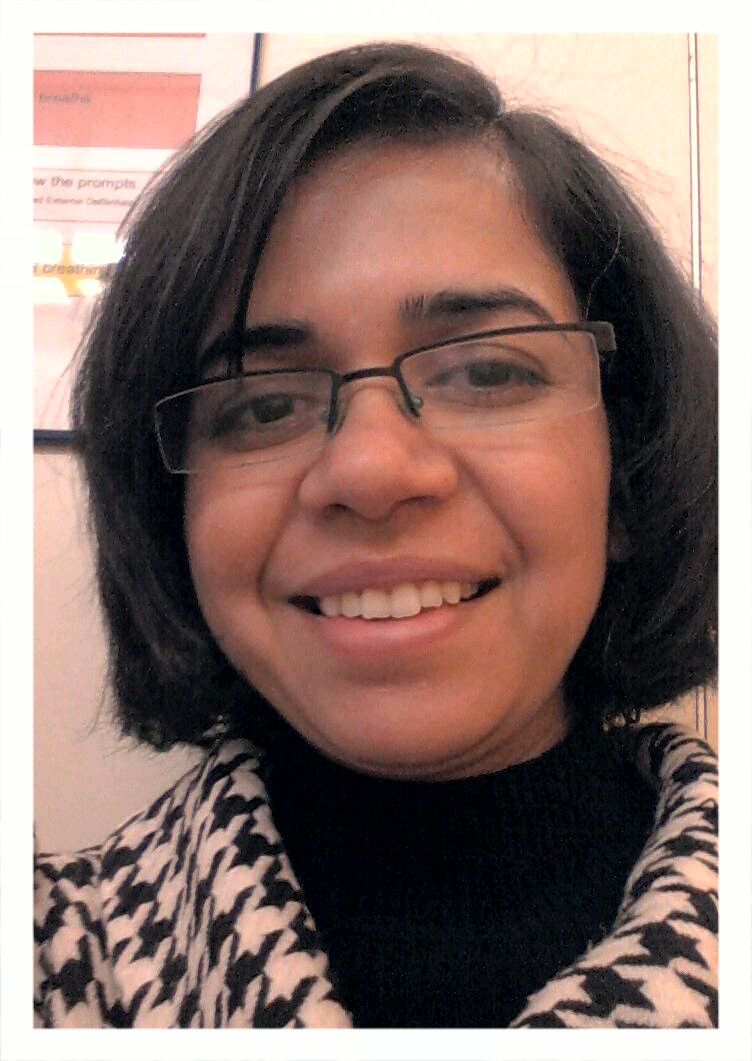
\includegraphics[width=\trainerIconWidth]{graphics/Tyagi.jpg} & 
      \textbf{Dr. Sonika Tyagi}\newline
      
      Senior Bioinformatics Officer\newline
      Australian Genome Research Facility Ltd, The Walter and Eliza Hall Institute, VIC\newline
      \mailto{sonika.tyagi@agrf.org.au}\\
    
    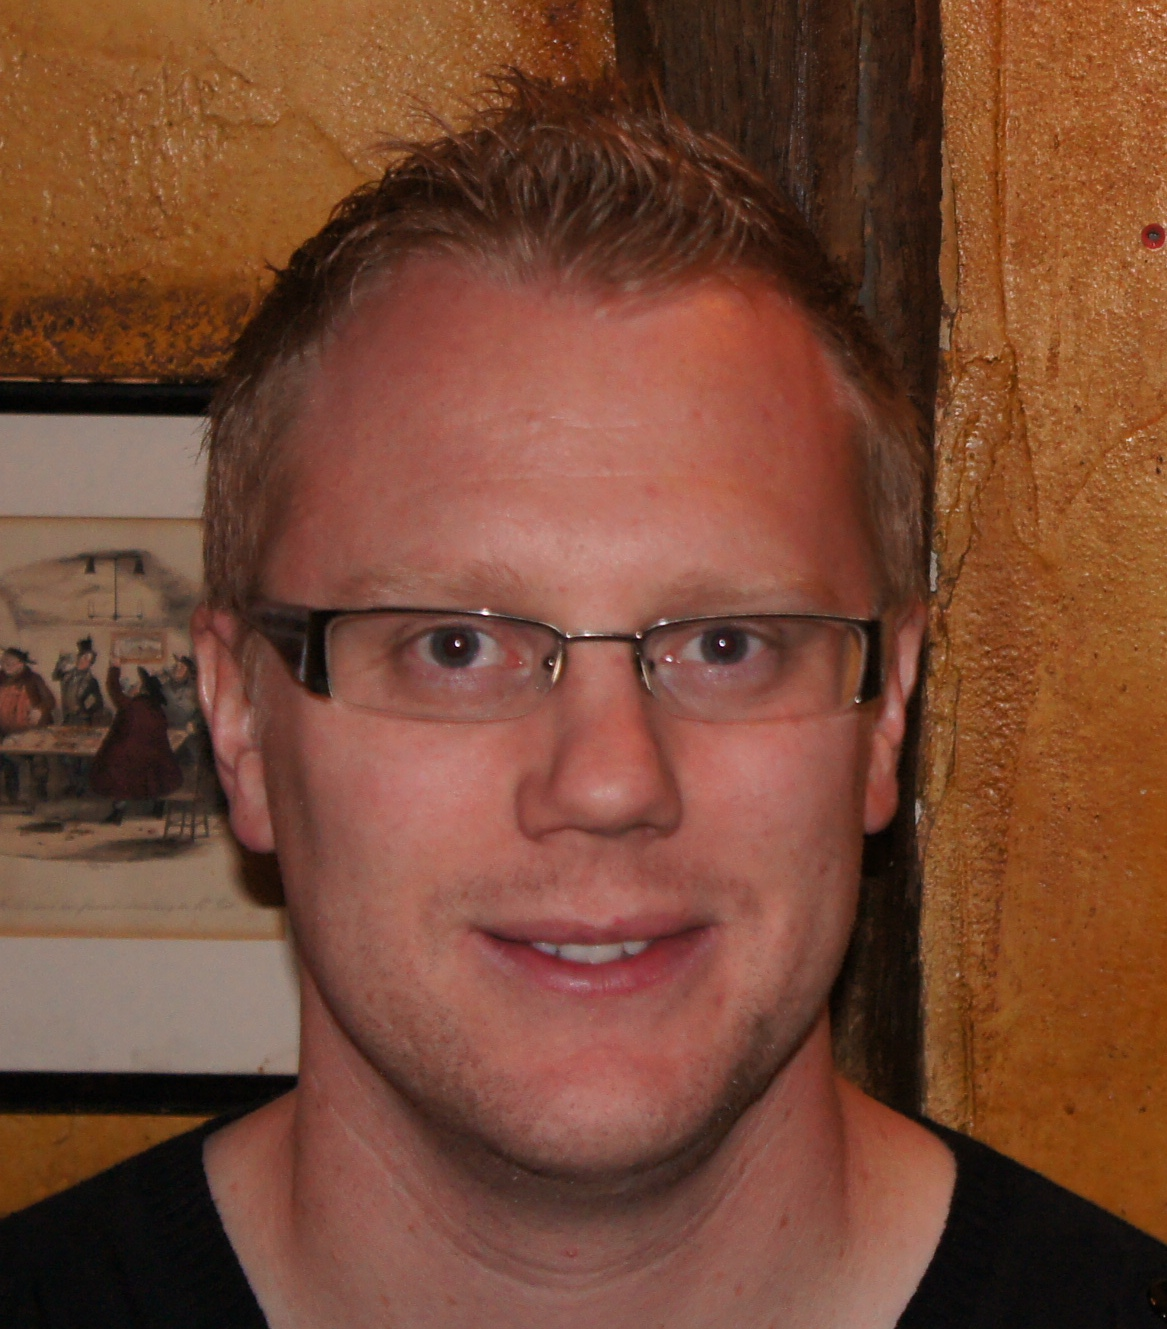
\includegraphics[width=\trainerIconWidth]{graphics/watson-haigh.jpeg} & 
      \textbf{Dr. Nathan S. Watson-Haigh}\newline
      
      Research Fellow in Bioinformatics\newline
      The Australian Centre for Plant Functional Genomics (ACPFG), SA\newline
      \mailto{nathan.haigh@acpfg.com.au}\\
    
    \end{tabular}
  \caption{\label{tab:trainers}}
\end{table}


%
% Workshop Preamble
%
%
% Start: General Information describing the workshop and the structure of the handouts
%
\newpage

% \section{Do's and Don'ts of the Workshop}
% TODO Add do's and don'ts e.g. email, social media etc 

\section{Document Structure}
We have provided you with an electronic copy of the workshop's hands-on tutorial documents.
We have done this for two reasons: 1) you will have something to take away with you at the 
end of the workshop, and 2) you can save time (mis)typing commands on the command line by using
copy-and-paste.

\begin{warning}
While you could fly through the hands-on sessions doing
copy-and-paste you will learn more if you take the time, saved from not having to type all those
commands, to understand what each command is doing!
\end{warning}

The commands to enter at a terminal look something like this:
\begin{lstlisting}
tophat --solexa-quals -g 2 --library-type fr-unstranded -j annotation/Danio_rerio.Zv9.66.spliceSites -o tophat/ZV9_2cells genome/ZV9 data/2cells_1.fastq data/2cells_2.fastq
\end{lstlisting}  

The following icons are used in the margin, throughout the documentation to help you locate:

% TODO limit the use of some icons throughout as some are clearly overused and confuse the eye
\hspace*{.2cm}\vcent{
\includegraphics[height=1cm]{./graphics/info.png}} Important\\
\hspace*{.2cm}\vcent{
\includegraphics[height=1cm]{./graphics/notes.png}} For reference\\
\hspace*{.2cm}\vcent{
\includegraphics[height=1cm]{./graphics/steps.png}} Follow these steps\\
\hspace*{.2cm}\vcent{
\includegraphics[height=1cm]{./graphics/questions.png}} Questions to answer\\
\hspace*{.2cm}\vcent{
\includegraphics[height=1cm]{./graphics/warning.png}} Warning - STOP and read\\
\hspace*{.2cm}\vcent{
\includegraphics[height=1cm]{./graphics/bonus1.png}} Bonus exercise for fast learners\\
\hspace*{.2cm}\vcent{
\includegraphics[height=1cm]{./graphics/bonus2.png}} Advanced exercise for super-fast learners\\

\section{Resources Used}
We have provided you with an environment which contains all the tools and data
you need for the duration of this workshop. However, we also provide details
about the tools and data used by each module at the start of the respective
module documentation.


%
% Start of modules
% Switch chapter styling to module
%
\chapterstyle{module}

%
% QC Module
%
% Define the top matter
\renewcommand{\moduleTitle}{Data Quality}
\renewcommand{\moduleAuthors}{%
  Sonika Tyagi \mailto{sonika.tyagi@agrf.org.au}
} \renewcommand{\moduleContributions}{%
  Nathan S. Watson-Haigh \mailto{nathan.watson-haigh@awri.com.au}%
}

%  Start: Module Title Page
\chapter{\moduleTitle}
\newpage
% End: Module Title Page

\section{Key Learning Outcomes}

After completing this practical the trainee should be able to:
\begin{itemize}
  \item Assess the overall quality of NGS sequence reads
  \item Visualise the quality, and other associated matrices, of reads to decide
        on filters and cutoffs for cleaning up data ready for downstream analysis
  \item Clean up and pre-process the sequences data for further analysis
\end{itemize}

\section{Resources You'll be Using}
 
\subsection{Tools Used}
\begin{description}[style=multiline,labelindent=0cm,align=left,leftmargin=0.5cm]
  \item[FastQC]\hfill\\
  	\url{http://www.bioinformatics.babraham.ac.uk/projects/fastqc/}
  \item[FASTX-Toolkit]\hfill\\
  	\url{http://hannonlab.cshl.edu/fastx_toolkit/}
  \item[Picard]\hfill\\
  	\url{http://picard.sourceforge.net/}
\end{description}

% \subsection{Sources of Data}
% TODO Provide a publically available data set used for this module
% \url{http://www.ebi.ac.uk/ena/data/view/ERR022484}\\
% \url{http://www.ebi.ac.uk/ena/data/view/ERR022485}

\newpage

\section{Introduction}

\begin{note}
Going on a blind date with your read set? For a better understanding of the
consequences please check the data quality!
\end{note}

For the purpose of this tutorial we are focusing only on Illumina sequencing
which uses 'sequence by synthesis' technology in a highly parallel fashion.
Although Illumina high throughput  sequencing provides highly accurate sequence
data, several sequence artefacts, including base calling errors and small
insertions/deletions, poor quality reads and primer/adapter contamination are
quite common in the high throughput sequencing data. The primary errors are
substitution errors. The error rates can vary from 0.5-2.0\% with errors mainly
rising in frequency at the 3' ends of reads.

One way to investigate sequence data quality is to visualize the quality scores
and other metrics in a compact manner to get an idea about the quality of a read
data set. Read data sets can be improved by post processing in different ways
like trimming off low quality bases, cleaning up any sequencing adapters and
removing PCR duplicates. We can also look at other statistics such
as, sequence length distribution, base composition, sequence complexity,
presence of ambiguous bases etc. to assess the overall quality of the data set.
Highly redundant coverage ($>$15X) of the genome can be used to correct sequencing
errors in the reads before assembly and errors. Various k-mer based error
correction methods exist but are beyond the scope of this tutorial.

\section{Prepare the Environment}

\begin{information}
To investigate sequence data quality we will demonstrate tools called FastQC
and FASTX-Toolkit. FastQC will process and present the reports in a visual manner.
Based on the results, the sequence data can be processed using the FASTX-Toolkit.
We will use one data set in this practical, which can be found in the QC
directory on your desktop.
\end{information}

\begin{steps}
Open the Terminal and go to the directory where the data are stored:
\begin{lstlisting}
cd ~/QC/
pwd
\end{lstlisting}

At any time, help can be displayed for FastQC using the following command:
\begin{lstlisting}
fastqc -h
\end{lstlisting}

\end{steps}


\section{Quality Visualisation}

\begin{information}
We have a file for a good quality and bad quality statistics. FastQC generates
results in the form of a zipped and unzipped directory for each input file.
\end{information}

\begin{steps}
Execute the following command on the two files:
\begin{lstlisting}
fastqc -f fastq bad_example.fastq 
fastqc -f fastq good_example.fastq
\end{lstlisting}

View the FastQC report file of the dab data using a web browser such as
firefox.

\begin{lstlisting}
firefox bad_example_fastqc/fastqc_report.html &
\end{lstlisting}

\end{steps}

\begin{note}
The report file will have a Basic Statistics table and various graphs and tables
for different quality statistics. E.g.:
\end{note}

% Table generated by Excel2LaTeX from sheet 'Sheet1'
\begin{table}[H]
  \centering
  \caption{FastQC Basic Statistics table}
    \begin{tabular}{ll}
    \toprule
    Filename & bad\_example.fastq \\
    \midrule
    File type & Conventional base calls \\
    Encoding & Sanger / Illumina 1.9 \\
    Total Sequences & 40000 \\
    Filtered Sequences & 0 \\
    Sequence length & 100 \\
    \%GC  & 48 \\
    \bottomrule
    \end{tabular}%
  \label{tab:badexampleuntrimmed}%
\end{table}%

\begin{figure}[H]
\centering
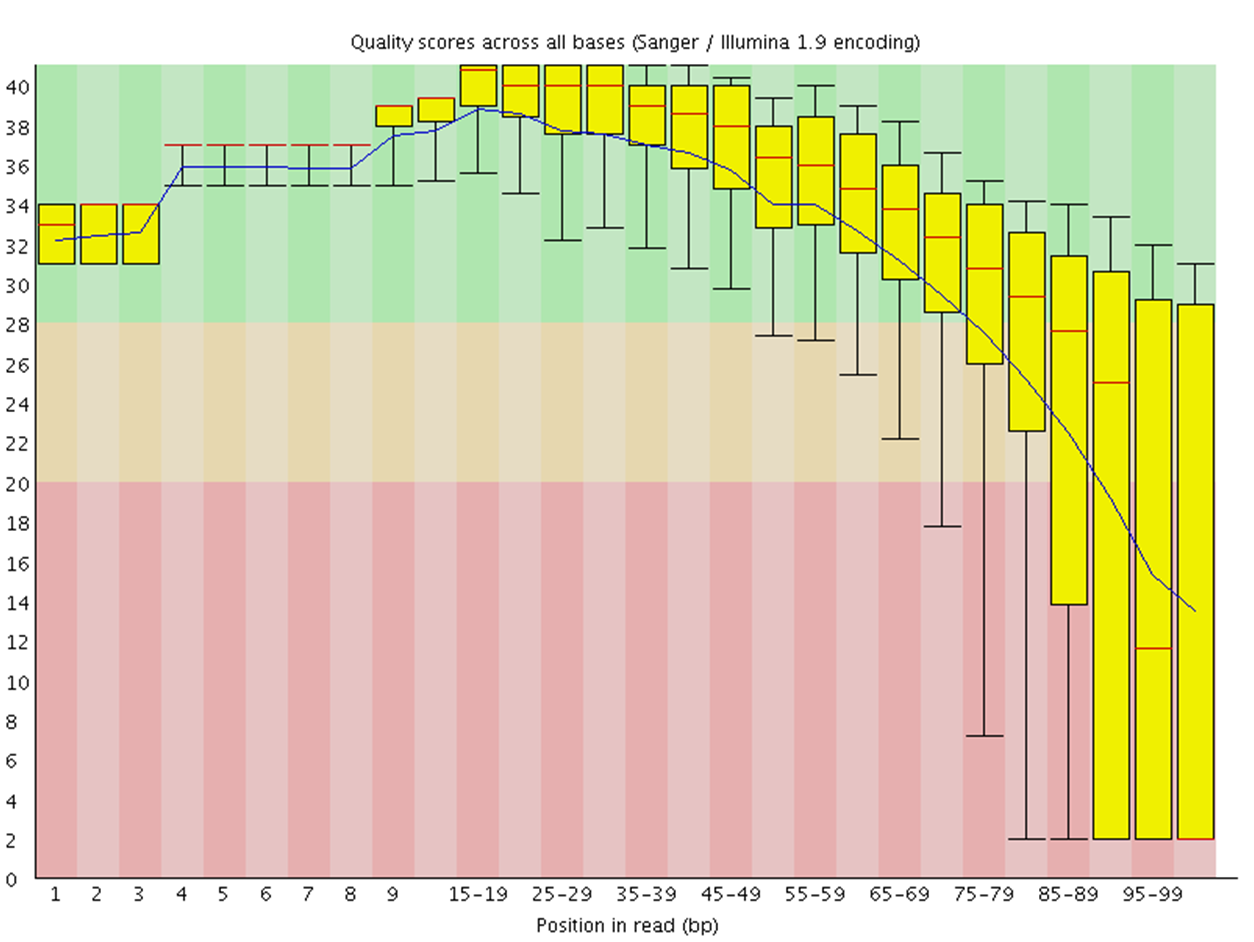
\includegraphics[width=0.8\textwidth]{ngs-qc/bad_example.png}
\caption{Per base sequence quality plot for \texttt{bad\_example.fastq}. Base positions in the reads are shown on x-axis and quality score (Q Score) are shown on the Y-axis}
\label{fig:bad_example_plot}
\end{figure}

\begin{information}
A quality score (or Q-score) expresses an error probability.  In particular, it
serves as a convenient and compact way to communicate very small error
probabilities.
Given an assertion, A, the probability that A is not true, $P(~ A)$, is expressed
by a quality score, $Q(A)$, according to the relationship:
\\\\
$Q(A) =-10 log10(P(\sim A))$
\\\\
Where $P(~ A)$ is the estimated probability of an assertion A being wrong.
The relationship between the quality score and error probability is demonstrated
with the following table:

% Table generated by Excel2LaTeX from sheet 'Sheet1'
\begin{table}[H]
  \centering
  \caption{Error probabilities associated with various quality (Q) values}
    \begin{tabular}{rr}
    \toprule
    \textbf{Quality score, Q(A)} & \textbf{Error probability, P($\sim$A)} \\
    \midrule
    10    & 0.1 \\
    20    & 0.01 \\
    30    & 0.001 \\
    40    & 0.0001 \\
    \bottomrule
    \end{tabular}%
  \label{tab:addlabel}%
\end{table}%

\end{information}

\begin{questions}
How many sequences were there in your file? What is the read length?
\begin{answer}
40,000. read length=100bp
\end{answer}

Does the quality score values vary throughout the read length?
(hint: look at the 'per base sequence quality plot')
\begin{answer}
Yes. Quality scores are dropping towards the end of the reads.
\end{answer}

What is the quality score range you see?
\begin{answer}
2-40
\end{answer}

At around which position do the scores start falling below Q20? 
\begin{answer}
Around 80 bp position
\end{answer}


How can we trim the reads to filter out the low quality data?
\begin{answer}
By trimming off the bases after a fixed position of the read. or by trimming off bases based on the quality score.
\end{answer}
\end{questions}

\begin{bonus}
\subsection{Good Quality Data}
View the FastQC report files fastqc\_report.html to see examples of a good
quality data and compare the quality plot with that of the bad\_example\_fastqc.

\begin{lstlisting}
firefox good_example_fastqc/fastqc_report.html &
\end{lstlisting}
\end{bonus}

\begin{note}
Sequencing errors can complicate the downstream analysis, which normally
requires that reads be aligned to each other (for genome assembly) or to a
reference genome (for detection of mutations). Sequence reads containing errors
may lead to ambiguous paths in the assembly or improper gaps. In variant
analysis projects sequence reads are aligned against the reference genome. The
errors in the reads may lead to more mismatches than expected from
mutations alone. But if these errors can be removed or corrected, the read
alignments and hence the variant detection will improve. The assemblies will also
improve after pre-processing the reads with errors.
\end{note}

\section{Read Trimming}
Read trimming can be done in a variety of different ways. Choose a method
which best suits your data. Here we are giving examples of fixed-length trimming
and quality-based trimming.

\subsection{Fixed Length Trimming}
Low quality read ends can be trimmed using a fixed-length timmer. We will use the
\texttt{fastx\_trimmer} from the FASTX-Toolkit. Usage message to find out various options
you can use with this tool. Type \fonttt{fastx\_trimmer -h} at anytime to display help.

\begin{steps}
We will no do fixed-length trimming of the \texttt{bad\_example.fastq} file
using the following command.
\begin{lstlisting}
cd ~/QC
fastx_trimmer -h
fastx_trimmer -Q 33 -f 1 -l 80 -i bad_example.fastq -o bad_example_trimmed01.fastq
\end{lstlisting}
\end{steps}

\begin{note}
We used the following options in the command above:
\begin{description}[style=multiline,labelindent=0cm,align=right,leftmargin=\descriptionlabelspace,rightmargin=1.5cm,font=\ttfamily]
 \item[-Q 33] Indicates the input quality scores are Phred+33 encoded
 \item[-f] First base to be retianed in the output
 \item[-l] Last base to be retained in the output
 \item[-i] Input fastq file name
 \item[-o] Output file name
\end{description}
\end{note}

\begin{steps}
Run FastQC on the trimmed file and visualise the quality scores of the trimmed file.
\begin{lstlisting}
fastqc -f fastq bad_example_trimmed01.fastq
firefox bad_example_trimmed01_fastqc/fastqc_report.html &
\end{lstlisting}

The output should look like:

\begin{table}[H]
  \centering
  \caption{FastQC Basic Statistics table}
    \begin{tabular}{ll}
    \toprule
    Filename & bad\_example\_trimmed01.fastq\\
    \midrule
    File type & Conventional base calls\\
    Encoding & Sanger / Illumina 1.9\\
    Total Sequences & 40000\\
    Filtered Sequences & 0\\
    Sequence length & 80\\
    \%GC & 48\\
    \bottomrule
    \end{tabular}%
  \label{tab:badexampletrimmed}%
\end{table}%

\begin{figure}[H]
\centering
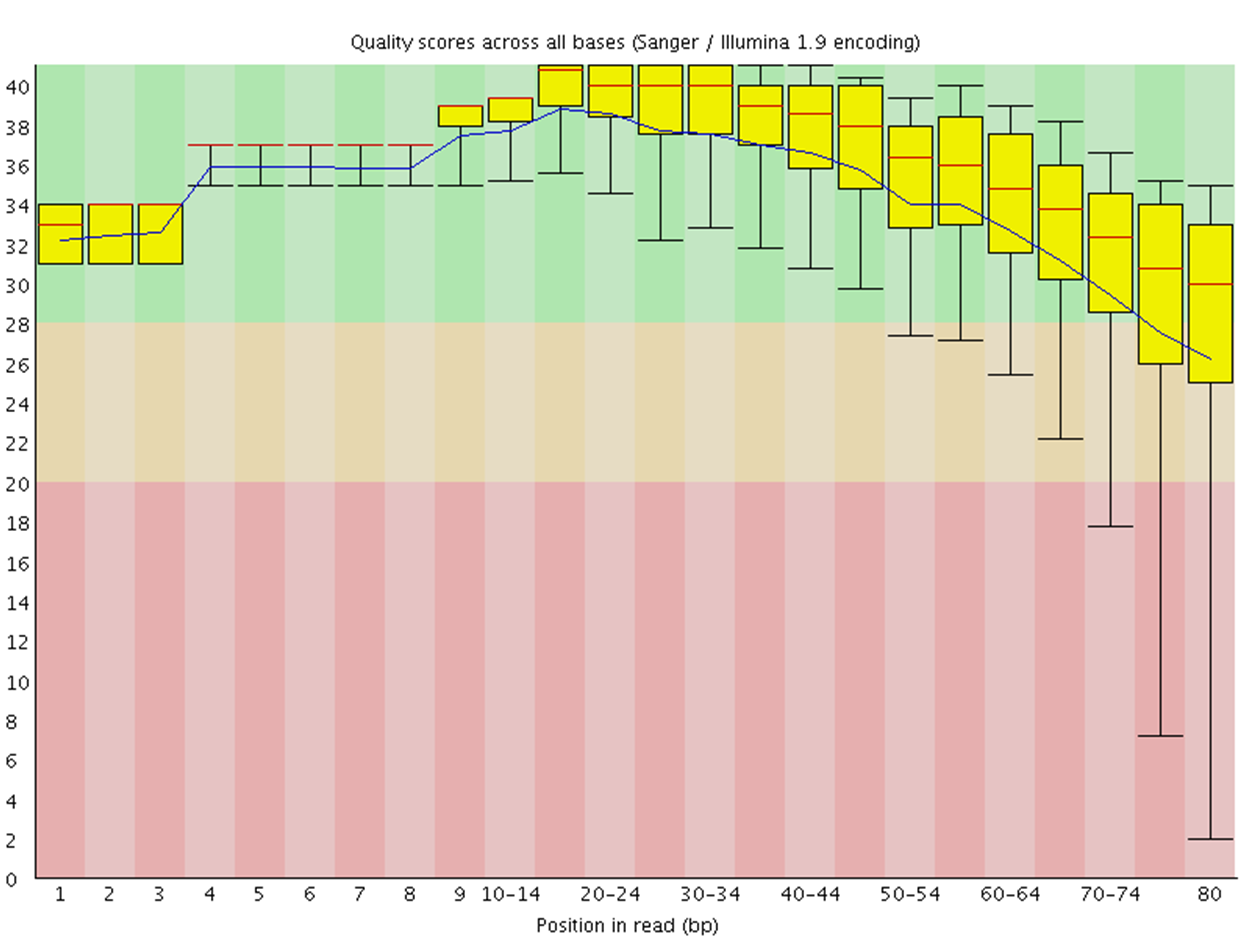
\includegraphics[width=0.8\textwidth]{ngs-qc/bad_example_trimmed_to_80bp.png}
\caption{Per base sequence quality plot for the fixed-length trimmed \texttt{bad\_example.fastq} reads. Base positions in the reads are shown on x-axis and quality score (Q Score) are shown on the Y-axis}
\label{fig:bad_example_trimmed_plot}
\end{figure}

\end{steps}

\begin{questions}
What values would you use for \texttt{-f} if you wanted to trim off 10 bases at
the 5' end of the reads?
\begin{answer}
\texttt{-f 11}
\end{answer}
\end{questions}

\subsection{Quality Based Trimming}
Base call quality scores can also be used to dynamically determine the trim points for each read. A quality
score threshold and minimum read length following trimming can be used to remove low
quality data.

\begin{steps}
Run the following command to quality trim your data:
\begin{lstlisting}
cd ~/QC
fastq_quality_trimmer -h
fastq_quality_trimmer -Q 33 -t 20 -l 50 -i bad_example.fastq -o bad_example_quality_trimmed.fastq
\end{lstlisting}
\end{steps}

\begin{steps}
Run FastQC on the quality trimmed file and visualise the quality scores.

\begin{lstlisting}
fastqc -f fastq bad_example_quality_trimmed.fastq
firefox bad_example_quality_trimmed_fastqc/fastqc_report.html &
\end{lstlisting}

The output should look like:

\begin{table}[H]
  \centering
  \caption{FastQC Basic Statistics table}
    \begin{tabular}{ll}
    \toprule
    Filename & bad\_example\_quality\_trimmed.fastq\\
    \midrule
    File type & Conventional base calls\\
    Encoding & Sanger / Illumina 1.9\\
    Total Sequences & 38976\\
    Filtered Sequences & 0\\
    Sequence length & 50-100\\
    \%GC & 48\\
    \bottomrule
    \end{tabular}%
  \label{tab:badexamplequalitytrimmed}%
\end{table}%

\begin{figure}[H]
\centering
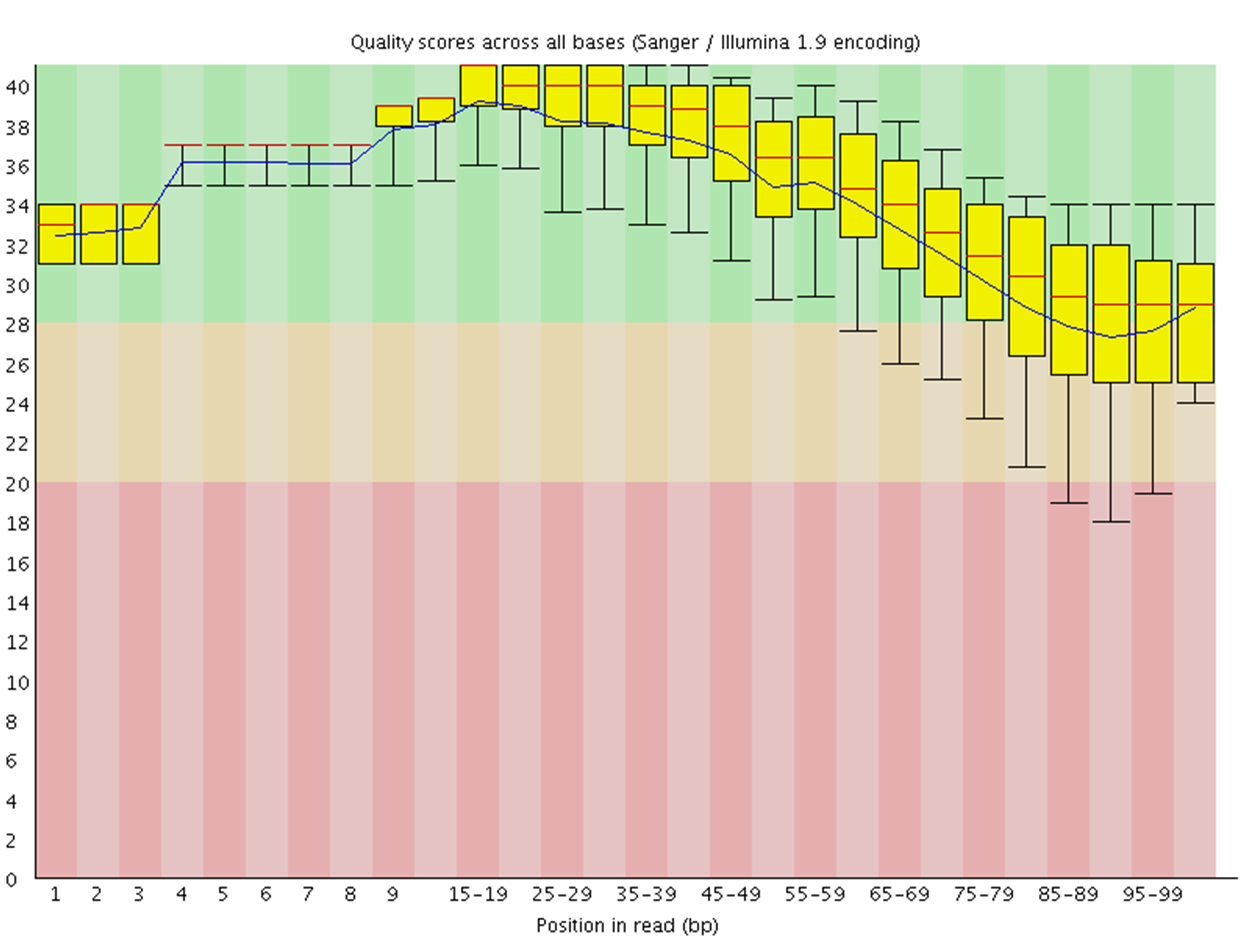
\includegraphics[width=0.8\textwidth]{ngs-qc/bad_example_quality_trimmed.png}
\caption{Per base sequence quality plot for the quality-trimmed \texttt{bad\_example.fastq} reads. Base positions in the reads are shown on x-axis and quality score (Q Score) are shown on the Y-axis}
\label{fig:bad_example_quality_trimmed_plot}
\end{figure}

\end{steps}

\begin{questions}
How did the quality score range change with two types of trimming?
\begin{answer}
Some poor quality bases (Q $<$20) are still present at the 3' end of the
fixed-length trimmed reads. It also removes bases that are good quality.

Quality-based trimming retains the 3' ends of reads which have good quality
scores.
\end{answer}

Did the number of total reads change after two types of trimming?
\begin{answer}
Quality trimming discarded $>$1000 reads. However, We retain a lot of maximal
length reads which have good quality all the way to the ends.
\end{answer}

What reads lengths were obtained after quality based trimming?
\begin{answer}
50-100

Reads $<$50 bp, following quality trimming, were discarded.
\end{answer}

Did you observe adapter sequences in the data?
\begin{answer}
No. (Hint: look at the overrepresented sequences.
\end{answer}

\end{questions}

\begin{advanced}
\subsection{Adapter Clipping}
Sometime sequence reads may end up getting the leftover of adapters and primers
used in the sequencing process. It's good practice to screen your data for
these possible contaminations for more sensitive alignment and assembly based
analysis.

\begin{note}
This is particularly important when read lengths can be longer than the
molecules being sequenced. For example when sequencing miRNAs.
\end{note}

Various QC tools are available to screen and/or clip these adapter/primer
sequences from your data. (e.g. FastQC, fastx, cutadapt).

\begin{steps}
Here we are demonstrating \texttt{fastx\_clipper} to trim a given adapter
sequence.

\begin{lstlisting}
cd ~/QC
fastx_clipper -h
fastx_clipper -v -Q 33 -l 20 -M 15 -a GATCGGAAGAGCGGTTCAGCAGGAATGCCGAG -i bad_example.fastq -o bad_example_clipped.fastq
\end{lstlisting}
\end{steps}

\begin{note}
An alternative tool, not installed on this system, for adapter clipping is
\texttt{fastq-mcf}. A list of adapters is provided in a text file. For more
information, see Fastqmcf at \url{http://code.google.com/p/ea-utils/wiki/FastqMcf}.
\end{note}

\subsection{Removing Duplicates}
Duplicate reads are the ones having the same start and end coordinates. This
may be the result of technical duplication (too many PCR cycles), or
over-sequencing (very high fold coverage). It is very important to put the
duplication level in context of your experiment. For example, duplication level
in targeted or re-sequencing projects may mean something different in RNA-seq
experiments. In RNA-seq experiments oversequencing is usually necessary when
detecting low abundance transcripts.

\begin{information}
The duplication level computed by FastQC is based on sequence identity at the
end of reads. Another tool, Picard, determines duplicates based on identical
start and end positions in SAM/BAM alignment files.

\textbf{We will not cover Picard but
provide the following for your information.}

Picard is a suite of tools for performing many common tasks with SAM/BAM format
files. For more information see the Picard website and information about the
various command-line tools available:

\url{http://picard.sourceforge.net/command-line-overview.shtml}
\end{information}

\begin{information}
Picard 1.69 is installed on this system in \texttt{/usr/share/java/picard-1.69/}

One of the Picard tools (MarkDuplicates) can be used to analyse and remove
duplicates from the raw sequence data. The input for Picard is a sorted
alignment file in BAM format. Short read aligners such as, bowtie, BWA and tophat
can be used to align FASTQ files against a reference genome to generate
SAM/BAM alignment format.
\end{information}

\begin{steps}
Interested users can use the following general command to run the
MarkDuplicates tool at their leisure and only need to provide a BAM file for
INPUT:


\begin{lstlisting}
cd ~/QC
java -jar /usr/share/java/picard/MarkDuplicates.jar INPUT=<alignment_file.bam> VALIDATION_STRINGENCY=LENIENT OUTPUT=alignment_file.dup METRICS_FILE=alignment_file.matric ASSUME_SORTED=true REMOVE_DUPLICATES=true

\end{lstlisting}
\end{steps}

\end{advanced}


%
% RNA-Seq Module
%
% Define the top matter
\setModuleTitle{RNA-Seq}
\setModuleAuthors{%
  Myrto Kostadima, EMBL-EBI \mailto{kostadmi@ebi.ac.uk}\\
  Remco Loos, EMBL-EBI \mailto{remco@ebi.ac.uk}
}
\setModuleContributions{%
  Nathan S. Watson-Haigh \mailto{nathan.watson-haigh@awri.com.au}%
}

%  Start: Module Title Page
\chapter{\moduleTitle}
\newpage
% End: Module Title Page

\section{Key Learning Outcomes}

After completing this practical the trainee should be able to:
\begin{itemize}
  \item Understand and perform a simple RNA-Seq analysis workflow.
  \item Perform gapped alignments to an indexed reference genome using TopHat.
  \item Perform transcript assembly using Cufflinks.
  \item Visualize transcript alignments and annotation in a genome browser such as IGV.
  \item Be able to identify differential gene expression between two experimental conditions.
\end{itemize}

\section{Resources You'll be Using}
 
\subsection{Tools Used}
\begin{description}[style=multiline,labelindent=0cm,align=left,leftmargin=1cm]
  \item[Tophat] \hfill\\
    \url{http://tophat.cbcb.umd.edu/}
  \item[Cufflinks] \hfill\\
    \url{http://cufflinks.cbcb.umd.edu/}
  \item[Samtools] \hfill\\
    \url{http://samtools.sourceforge.net/}
  \item[BEDTools] \hfill\\
    \url{http://code.google.com/p/bedtools/}
  \item[UCSC tools] \hfill\\
    \url{http://hgdownload.cse.ucsc.edu/admin/exe/}
  \item[IGV] \hfill\\
    \url{http://www.broadinstitute.org/igv/}
  \item[DAVID Functional Analysis] \hfill\\
    \url{http://david.abcc.ncifcrf.gov/}
\end{description}

\subsection{Sources of Data}
\url{http://www.ebi.ac.uk/ena/data/view/ERR022484}\\
\url{http://www.ebi.ac.uk/ena/data/view/ERR022485}

\newpage

\section{Introduction}
The goal of this hands-on session is to perform some basic tasks in the
downstream analysis of RNA-seq data. We will start from RNA-seq data aligned to
the zebrafish genome using Tophat.

We will perform transcriptome reconstruction using Cufflinks and we will compare
the gene expression between two different conditions in order to identify
differentially expressed genes.

\section{Prepare the Environment}
We will use a dataset derived from sequencing of mRNA from \textit{Danio rerio} embryos
in two different developmental stages. Sequencing was performed on the Illumina
platform and generated 76bp paired-end sequence data using polyA selected RNA.
Due to the time constraints of the practical we will only use a subset of the
reads.

The data files are contained in the subdirectory called \texttt{data} and are
the following:
\begin{description}[style=multiline,labelindent=1.5cm,align=left,leftmargin=2.5cm]
  \item[\texttt{2cells\_1.fastq} and \texttt{2cells\_2.fastq}] \hfill\\
 These files are based on RNA-seq data of a 2-cell zebrafish embryo
  \item[\texttt{6h\_1.fastq} and \texttt{6h\_2.fastq}] \hfill\\
 These files are based on RNA-seq data of zebrafish embryos 6h post
 fertilization
\end{description}

\begin{steps}
Open the Terminal and go to the \texttt{RNA-seq} working directory:
\begin{lstlisting}
cd ~/RNA-seq/
\end{lstlisting}
\end{steps}

%\reversemarginpar\marginpar{\vskip+0em\hfill
\includegraphics[height=1cm]{./graphics/warning.png}}
%\textcolor{red}{
\begin{warning}
  All commands entered into the terminal for this tutorial should be from within the
  \textbf{\texttt{$\sim$/RNA-seq}} directory.
\end{warning}

\begin{steps}
Check that the \texttt{data} directory contains the above-mentioned files by typing:
\begin{lstlisting}
ls data
\end{lstlisting}
\end{steps}

\section{Alignment}
There are numerous tools for performing short read alignment and the choice of aligner
should be carefully made according to the analysis goals/requirements. Here we will
use Tophat, a widely used ultrafast aligner that performs spliced alignments.

Tophat is based on the Bowtie aligner and uses an indexed genome for the
alignment to speed up the alignment and keep its memory footprint small. 
The the index for the \textit{Danio rerio} genome has been created for you. 

\begin{warning}
The commands to create an index follow, do not run
\begin{lstlisting}
bowtie-build genome/Danio_rerio.Zv9.66.dna.fa genome/ZV9
\end{lstlisting}
\end{warning}

\begin{steps}
Tophat has a number of parameters in order to perform the alignment. To view them all type:
\begin{lstlisting}
tophat --help
\end{lstlisting}
\end{steps}

\begin{information}
The general format of the tophat command is:
\begin{lstlisting}[style=command_syntax]
tophat [options]* <index_base> <reads_1> <reads_2>
\end{lstlisting}

Where the last two arguments are the \texttt{.fastq} files of the paired end
reads, and the argument before is the basename of the indexed genome.
\end{information}

\begin{note}
The quality values in the FASTQ files used in this hands-on session are Phred+33
encoded. We explicitly tell tophat of this fact by using the command line
argument \texttt{--solexa-quals}.
\end{note}

\begin{information}
You can look at the first few reads in the file \texttt{data/2cells\_1.fastq} with:
 
\begin{lstlisting}
head -n 20 data/2cells_1.fastq
\end{lstlisting}
\end{information}

%\reversemarginpar\marginpar{\vskip+0em\hfill
\includegraphics[height=1cm]{./graphics/notes.png}}
\begin{note}
Some other parameters that we are going to use to run Tophat are listed below:
\begin{description}[style=multiline,labelindent=0cm,align=right,leftmargin=\descriptionlabelspace,rightmargin=1.5cm,font=\ttfamily]
 \item[-g] Maximum number of multihits allowed. Short reads are likely to map to
 more than one location in the genome even though these reads can have originated
 from only one of these regions. In RNA-seq we allow for a limited number of
 multihits, and in this case we ask Tophat to report only reads that map at most
 onto 2 different loci.
 \item[--library-type] Before performing any type of RNA-seq analysis you need
 to know a few things about the library preparation. Was it done using a
 strand-specific protocol or not? If yes, which strand? In our data the protocol
 was NOT strand specific.
 \item[-j] Improve spliced alignment by providing Tophat with annotated splice
 junctions. Pre-existing genome annotation is an advantage when analysing RNA-seq
 data. This file contains the coordinates of annotated splice junctions from Ensembl.
 These are stored under the sub-directory \texttt{annotation} in a file called
 \texttt{ZV9.spliceSites}.
 \item[-o] This specifies in which subdirectory Tophat should save the output
 files. Given that for every run the name of the output files is the same, we
 specify different directories for each run.
\end{description}
\end{note}

It takes some time (approx. 20 min) to perform tophat spliced alignments, even for this subset of
reads. Therefore, we have pre-aligned the \texttt{2cells} data for you using the following command:
\begin{warning}
You DO NOT need to run this command yourself - we have done this for you.

\begin{lstlisting}
tophat --solexa-quals -g 2 --library-type fr-unstranded -j annotation/Danio_rerio.Zv9.66.spliceSites -o tophat/ZV9_2cells genome/ZV9 data/2cells_1.fastq data/2cells_2.fastq
\end{lstlisting}
\end{warning}

\begin{steps}
Align the \texttt{6h} data yourself using the following command:  

\begin{lstlisting}
# Takes approx. 20mins
tophat --solexa-quals -g 2 --library-type fr-unstranded -j annotation/Danio_rerio.Zv9.66.spliceSites -o tophat/ZV9_6h genome/ZV9 data/6h_1.fastq data/6h_2.fastq
\end{lstlisting}

\end{steps}

The \texttt{6h} read alignment will take approx. 20 min to complete. Therefore,
we'll take a look at some of the files, generated by tophat, for the
pre-computed \texttt{2cells} data.

\subsection{Alignment Visualisation in IGV}

The Integrative Genomics Viewer (IGV) is able to provide a visualisation of read
alignments given a reference sequence and a BAM file. We'll visualise the
information contained in the \texttt{accepted\_hits.bam} and
\texttt{junctions.bed} files for the pre-computed \texttt{2cells} data. The
former, contains the tophat sliced alignments of the reads to the reference
while the latter stores the coordinates of the splice junctions present in the
data set.

\begin{steps}
Open the \texttt{RNA-seq} directory on your Desktop and double-click the
\texttt{tophat} subdirectory and then the \texttt{ZV9\_2cells} directory.

\begin{enumerate}
  \item Launch IGV by double-clicking the ``IGV 2.3'' icon on the Desktop
  (ignore any warnings that you may get as it opens). \emph{NOTE: IGV may take
  several minutes to load for the first time, please be patient.}
  \item Choose ``Zebrafish (Zv9)'' from the drop-down box in the top left of the
  IGV window. Else you can also load the genome fasta file.
  \item Load the \texttt{accepted\_hits.sorted.bam} file by clicking the
  ``File'' menu, selecting ``Load from File'' and navigating to the
  \texttt{Desktop/RNA-seq/tophat/ZV9\_2cells} directory.
  \item Rename the track by right-clicking on its name and choosing ``Rename
  Track''. Give it a meaningful name like ``2cells BAM''.
  \item Load the \texttt{junctions.bed} from the same directory and rename the
  track ``2cells Junctions BED''.
  \item Load the Ensembl annotations file \texttt{Danio\_rerio.Zv9.66.gtf}
  stored in the \texttt{RNA-seq/annotation} directory.
  \item Navigate to a region on chromosome 12 by typing
  \texttt{chr12:20,270,921-20,300,943} into the search box at the top of the IGV
  window.
\end{enumerate}

\end{steps}

\begin{information}
Keep zooming to view the bam file alignments

Some useful IGV manuals can be found below

http://www.broadinstitute.org/software/igv/interpreting_insert_size
http://www.broadinstitute.org/software/igv/alignmentdata
\end{information}


\begin{questions}
Can you identify the splice junctions from the BAM file?
\begin{answer}
Slice junctions can be identified in the alignment BAM files.
These are the aligned RNA-Seq reads that have skipped-bases from the reference genome (most likely introns).
\end{answer}

Are the junctions annotated for \texttt{CBY1} consistent with the annotation?
\begin{answer}
Read alignment supports an extended length in exon 5 to the gene model (cby1-001) 
\end{answer}

Are all annotated genes, from both RefSeq and Ensembl, expressed?
\begin{answer}
No BX000473.1-201 is not expressed
\end{answer}

\end{questions}

\begin{steps}
Once tophat finishes aligning the 6h data you will need to sort the alignments found in the BAM file and then index the
sorted BAM file.

\begin{lstlisting}
samtools sort tophat/ZV9_6h/accepted_hits.bam tophat/ZV9_6h/accepted_hits.sorted
samtools index tophat/ZV9_6h/accepted_hits.sorted.bam
\end{lstlisting}

Load the sorted BAM file into IGV, as described previously, and rename the track appropriately.
\end{steps}

\newpage
\section{Isoform Expression and Transcriptome Assembly}
There are a number of tools that perform reconstruction of the transcriptome
and for this workshop we are going to use Cufflinks. Cufflinks can do
transcriptome assembly either \textit{ab initio} or using a reference annotation. It
also quantifies the isoform expression in Fragments
Per Kilobase of exon per Million fragments mapped (FPKM).

\begin{steps}
Cufflinks has a number of parameters in order to perform transcriptome
assembly and quantification. To view them all type:

\begin{lstlisting}
cufflinks --help
\end{lstlisting}
\end{steps}

We aim to reconstruct the transcriptome for both samples by using the Ensembl
annotation both strictly and as a guide. In the first case Cufflinks will only
report isoforms that are included in the annotation, while in the latter case
it will report novel isoforms as well.

The Ensembl annotation for \textit{Danio rerio} is available in
\texttt{annotation/Danio\_rerio.Zv9.66.gtf}.

\begin{information}
The general format of the \texttt{cufflinks} command is:
\begin{lstlisting}[style=command_syntax]
cufflinks [options]* <aligned_reads.(sam|bam)>
\end{lstlisting}
Where the input is the aligned reads (either in SAM or BAM format).
\end{information}

\begin{note}
Some of the available parameters for Cufflinks that we are going to use to run
Cufflinks are listed below:
\begin{description}[style=multiline,labelindent=0cm,align=right,leftmargin=\descriptionlabelspace,rightmargin=1.5cm,font=\ttfamily]
  \item[-o] Output directory.
  \item[-G] Tells Cufflinks to use the supplied GTF annotations strictly in order
  to estimate isoform annotation.
  \item[-b] Instructs Cufflinks to run a bias detection and correction algorithm
  which can significantly improve accuracy of transcript abundance estimates.
  To do this Cufflinks requires a multi-fasta file with the genomic sequences
  against which we have aligned the reads.
  \item[-u] Tells Cufflinks to do an initial estimation procedure to more
  accurately weight reads mapping to multiple locations in the genome
  (multi-hits).
  \item[--library-type] Before performing any type of RNA-seq analysis you need
  to know a few things about the library preparation. Was it done using a
  strand-specific protocol or not? If yes, which strand? In our data the protocol
  was NOT strand specific.
\end{description}
\end{note}

\begin{steps}
Perform transcriptome assembly, strictly using the supplied GTF annotations, for the \texttt{2cells} and \texttt{6h} data using cufflinks:
\begin{lstlisting}
# 2cells data (takes approx. 5mins):
cufflinks -o cufflinks/ZV9_2cells_gtf -G annotation/Danio_rerio.Zv9.66.gtf -b genome/Danio_rerio.Zv9.66.dna.fa -u --library-type fr-unstranded tophat/ZV9_2cells/accepted_hits.bam
# 6h data (takes approx. 5mins):
cufflinks -o cufflinks/ZV9_6h_gtf -G annotation/Danio_rerio.Zv9.66.gtf -b genome/Danio_rerio.Zv9.66.dna.fa -u --library-type fr-unstranded tophat/ZV9_6h/accepted_hits.bam
\end{lstlisting}
\end{steps}

\begin{information}
Cufflinks generates several files in the specified output directory. Here's a short description of these files:

\begin{description}[style=multiline,labelindent=0cm,align=right,leftmargin=\descriptionlabelspace,rightmargin=1.5cm,font=\ttfamily]
\item[genes.fpkm\_tracking] Contains the estimated gene-level expression values.
\item[isoforms.fpkm\_tracking] Contains the estimated isoform-level expression values.
\item[skipped.gtf] Contains loci skipped as a result of exceeding the maximum number of fragments.
\item[transcripts.gtf] This GTF file contains Cufflinks' assembled isoforms.
\end{description}

The complete documentation can be found at:
\url{http://cufflinks.cbcb.umd.edu/manual.html#cufflinks_output}
\end{information}

\begin{information}
So far we have forced cufflinks, by using the \texttt{-G} option, to strictly
use the GTF annotations provided and thus novel transcripts will not be reported. We
can get cufflinks to perform a GTF-guided transcriptome assembly by using the
\texttt{-g} option instead. Thus, novel transcripts will be reported.

\end{information}

\begin{warning}
GTF-guided transcriptome assembly is more computationally intensive than
strictly using the GTF annotations. Therefore, we have pre-computed these
GTF-guided assemblies for you and have placed the results under subdirectories:
\texttt{cufflinks/ZV9\_2cells\_gtf\_guided} and
\texttt{cufflinks/ZV9\_6h\_gft\_guided}.

You DO NOT need to run these commands. We provide them so you know how we
generated the the GTF-guided transcriptome assemblies:
\begin{lstlisting}
# 2cells guided transcriptome assembly (takes approx. 30mins):
cufflinks -o cufflinks/ZV9_2cells_gtf_guided -g annotation/Danio_rerio.Zv9.66.gtf -b genome/Danio_rerio.Zv9.66.dna.fa -u --library-type fr-unstranded tophat/ZV9_2cells/accepted_hits.bam
# 6h guided transcriptome assembly (takes approx. 30mins):
cufflinks -o cufflinks/ZV9_6h_gtf_guided -g annotation/Danio_rerio.Zv9.66.gtf -b genome/Danio_rerio.Zv9.66.dna.fa -u --library-type fr-unstranded tophat/ZV9_6h/accepted_hits.bam
\end{lstlisting}

\end{warning}

\begin{steps}
\begin{enumerate}
  \item Go back to IGV and load the pre-computed, GTF-guided transcriptome
  assembly for the \texttt{2cells} data
  (\texttt{cufflinks/ZV9\_2cells\_gtf\_guided/transcripts.gtf}).
  \item Rename the track as ``2cells GTF-Guided Transcripts''.
  \item In the search box type \texttt{ENSDART00000082297} in order for the
  browser to zoom in to the gene of interest.
\end{enumerate}
\end{steps}

\begin{questions}
Do you observe any difference between the Ensembl GTF annotations and the
GTF-guided transcripts assembled by cufflinks (the ``2cells GTF-Guided Transcripts'' track)?
\begin{answer}
Yes. It appears that the Ensembl annotations may have truncated the last exon.
However, our data also doesn't contain reads that span between the last two
exons.
\end{answer}

\end{questions}

\section{Differential Expression}
One of the stand-alone tools that perform differential expression analysis is
Cuffdiff. We use this tool to compare between two conditions; for example
different conditions could be control and disease, or wild-type and mutant, or
various developmental stages.

In our case we want to identify genes that are
differentially expressed between two developmental stages; a \texttt{2cells}
embryo and \texttt{6h} post fertilization.

\begin{information}
The general format of the cuffdiff command is:
\begin{lstlisting}[style=command_syntax]
cuffdiff [options]* <transcripts.gtf> <sample1_replicate1.sam[,...,sample1_replicateM]> <sample2_replicate1.sam[,...,sample2_replicateM.sam]>
\end{lstlisting}

Where the input includes a \texttt{transcripts.gtf} file, which is an annotation
file of the genome of interest, and the aligned reads (either in SAM or BAM
format) for the conditions.
Some of the Cufflinks options that we will use to run the program are:
\begin{description}[style=multiline,labelindent=0cm,align=right,leftmargin=\descriptionlabelspace,rightmargin=1.5cm,font=\ttfamily]
  \item[-o] Output directory.
  \item[-L] Labels for the different conditions
  \item[-T] Tells Cuffdiff that the reads are from a time series experiment.
  \item[-b] Instructs Cufflinks to run a bias detection and correction algorithm
  which can significantly improve accuracy of transcript abundance estimates.
  To do this Cufflinks requires a multi-fasta file with the genomic sequences
  against which we have aligned the reads.
  \item[-u] Tells Cufflinks to do an initial estimation procedure to more
  accurately weight reads mapping to multiple locations in the genome
  (multi-hits). 
  \item[--library-type] Before performing any type of RNA-seq analysis you need
 to know a few things about the library preparation. Was it done using a
 strand-specific protocol or not? If yes, which strand? In our data the protocol
 was NOT strand specific.
\end{description}
\end{information}

\begin{steps}
Run cuffdiff on the cufflinks generated BAM files for the 2cells vs. 6h data sets:
\begin{lstlisting}
cuffdiff -o cuffdiff/ -L ZV9_2cells,ZV9_6h -T -b genome/Danio_rerio.Zv9.66.dna.fa -u --library-type fr-unstranded annotation/Danio_rerio.Zv9.66.gtf tophat/ZV9_2cells/accepted_hits.bam tophat/ZV9_6h/accepted_hits.bam
\end{lstlisting}
\end{steps}

\begin{steps}
We are interested in the differential expression at the gene level. The results
are reported by Cuffdiff in the file \texttt{cuffdiff/gene\_exp.diff}. 
Look at the first few lines of the file using the following command:
\begin{lstlisting}
head -n 20 cuffdiff/gene_exp.diff
\end{lstlisting}

We would like to see which are the most significantly differentially expressed
genes. Therefore we will sort the above file according to the q value
(corrected p value for multiple testing). The result will be stored in a
different file called \texttt{gene\_exp\_qval.sorted.diff}.
\begin{lstlisting}
sort -t$'\t' -g -k 13 cuffdiff/gene_exp.diff > cuffdiff/gene_exp_qval.sorted.diff
\end{lstlisting}

Look again at the first few lines of the sorted file by typing:
\begin{lstlisting}
head -n 20 cuffdiff/gene_exp_qval.sorted.diff
\end{lstlisting}

Copy an Ensembl transcript identifier from the first two columns for one of
these genes (e.g. \texttt{ENSDARG00000077178}). Now go back to the IGV browser
and paste it in the search box.
\end{steps}

\begin{questions}
Do you see any difference in the read coverage between the \texttt{2cells} and
\texttt{6h} conditions that might have given rise to this transcript being
called as differentially expressed?
\begin{warning}
Note that the coverage on the Ensembl browser is based on raw reads and no
normalisation has taken place contrary to the FPKM values.
\end{warning}

\begin{answer}
The read coverage of this transcript (\texttt{ENSDARG00000077178}) in the 2cells
data set is much higher than in the 6h data set.
\end{answer}

\end{questions}

\begin{bonus}
\section{Functional Annotation of Differentially Expressed Genes}
After you have performed the differential expression analysis you are interested
in identifying if there is any functionality enrichment for your differentially
expressed genes.
On your Desktop click:
\begin{lstlisting}[style=command_syntax]
Applications >> Internet >> Firefox Web Browser
\end{lstlisting}
And go to the following URL: \url{http://david.abcc.ncifcrf.gov/}
On the left side click on Functional Annotation. Then click on the Upload tab.
Under the section Choose from File, click Choose File and navigate to the
\texttt{cuffdiff} directory. Select the file called \texttt{globalDiffExprs\_Genes\_qval.01\_top100.tab}.
Under Step 2 select ENSEMBL\_GENE\_ID from the drop-down menu. Finally select
Gene list and then press Submit List.
Click on Gene Ontology and then click on the CHART button of the GOTERM\_BP\_ALL item.

\begin{questions}
Do these categories make sense given the samples we're studying?
\begin{answer}
Developmental Biology
\end{answer}

Browse around DAVID website and check what other information are available.
\begin{answer}
Cellular component, Molecular function, Biological Processes, Tissue expression, Pathways, Literature, Protein domains 
\end{answer}
\end{questions}
\end{bonus}

\newpage

\section{References}
%TODO Change to using BiBTeX
\begin{enumerate}
  \item Trapnell, C., Pachter, L. \& Salzberg, S. L. TopHat: discovering splice
  junctions with RNA-Seq. Bioinformatics 25, 1105-1111 (2009).
  \item Trapnell, C. et al. Transcript assembly and quantification by RNA-Seq
  reveals unannotated transcripts and isoform switching during cell
  differentiation. Nat. Biotechnol. 28, 511-515 (2010).
  \item Langmead, B., Trapnell, C., Pop, M. \& Salzberg, S. L. Ultrafast and
  memory-efficient alignment of short DNA sequences to the human genome.
  Genome Biol. 10, R25 (2009).
  \item Roberts, A., Pimentel, H., Trapnell, C. \& Pachter, L. Identification
  of novel transcripts in annotated genomes using RNA-Seq. Bioinformatics 27,
  2325-2329 (2011).
  \item Roberts, A., Trapnell, C., Donaghey, J., Rinn, J. L. \& Pachter, L.
  Improving RNA-Seq expression estimates by correcting for fragment bias.
  Genome Biol. 12, R22 (2011).
\end{enumerate}


%
% End of modules
% Switch back to normal workshop chapter styling
%
\chapterstyle{workshop}

\chapter{Post-Workshop Information}
\clearpage
%
% Access to Computational Resources
%
\section{Access to Computational Resources}

By the end of the workshop we hope you're thinking one or more of the following:

\begin{itemize}
\item I'm interested in dabbling some more during my day-job!
\item How do I access a Linux box like the one I've been using in the workshop -
I \emph{really} don't want the hassle of setting this all up myself!
\item I'm hooked! I \emph{really} want to get down and dirty with NGS data! What
computational resources do I need, what do I have access to and how do I access
them?
\end{itemize}

We're ecstatic you're thinking this way and want to help guide you! However, lets
take this one step at a time.

The quickest way to dabble is to use a clone of the operating system (OS) you've
been using during this workshop. That means you'll have hassle-free access to a
plethora of pre-installed, pre-configured bioinformatics tools. You could even set it
up to contain a copy of all the workshop data and handouts etc to go through the
hands-on practicals in your own time!

We have created an image file (approx. 10 GBytes in size) of the NGS Training OS for you to
use as you wish:
\\\\
%\url{https://swift.rc.nectar.org.au:8888/v1/AUTH_809/NGSImage/NGSTrainingV1.0.vdi}
\url{https://swift.rc.nectar.org.au:8888/v1/AUTH_33065ff5c34a4652aa2fefb292b3195a/VMs/NGSTrainingV1.2.1.vdi}
\\\\
We would advise one of the following two approaches for making use of it:

\begin{itemize}
\item Import it into VirtualBox to setup a virtual machine (VM) on your own
computer.
\item Instantiate a VM on the NeCTAR Research Cloud.
\end{itemize}

\subsection{Setting up a VM using VirtualBox}
This approach requires the least amount of mind-bending to get up and running.
However, you will need to install some software. If you do not have
administrator access or your system administrator is slow or unwilling to
install the software, you may find using the NeCTAR Research Cloud to be viable
alternative.

This approach will use, at most, the computational resources available on
your own computer. If you are analysing non-microbial organisms or performing
\textit{de novo} assemblies, you may find these resources are insufficient. If this is the
case, you really should speak to someone from IT support at your institution or
get in touch with a bioinformatician for advise.

The software you need is VirtualBox, a freely available, Open Source
virtualisation product from Oracle (\url{https://www.virtualbox.org/}). This
software essentially allows you to run an operating system (the guest OS) within
another (the host OS). VirtualBox is available for several different host OSes
including MS Windows, OS X, Linux and Solaris
(\url{https://www.virtualbox.org/wiki/Downloads}). Once VirtualBox is installed
on your host OS, you can then install a guest OS inside VirtualBox. VirtualBox
supports a lot of different OSes
(\url{https://www.virtualbox.org/wiki/Guest_OSes}).

Here are the steps to setting up a VM in VirtualBox with our image file:
\begin{enumerate}
  \item Download and install VirtualBox for your OS: 
  \url{https://www.virtualbox.org/wiki/Downloads}
  \item Start VirtualBox and click New to start the Create New Virtual Machine wizard
  \item Give the VM a useful name like ``NGS Training'' and choose Linux and
  either Ubuntu or Ubuntu (64-bit) as the OS Type
  \item Give the VM access to a reasonable amount of the host Oses memory. i.e.
  somewhere near the top of the green. If this value is $<$ 2000 MB, you are
  likely to have insufficient memory for your NGS data analysis needs.
  \item For the virtual hard disk, select ``Use existing hard disk'' and browse
  to and select the \texttt{NGSTrainingV1.2.1.vdi} file you downloaded.
  \item Confirm remaining settings
  \item Select the ``NGS Training'' VM and click Start to boot he machine.
  \item Once booted, log into the VM as either \texttt{ubuntu} (a sudoer user;
  i.e. has admin rights) or as \texttt{ngstrainee} (a regular unprivileged
  user). See table below for passwords.
\end{enumerate}


\subsection{Setting up a VM using the NeCTAR Research Cloud}
All Australian researchers, who are members of an institution which subscribes
to the Australian Access Federation (AAF; \url{http://www.aaf.edu.au/}), have
access to a small amount of computing resources (2 CPU's and 8 GBytes RAM) on
the NeCTAR Research Cloud (\url{http://nectar.org.au/research-cloud}).

\subsubsection{Login to the NeCTAR Research Cloud Dashboard}
The online dashboard is a graphical interface for administering (creating,
deleting, rebooting etc) your virtual machines (VMs) on the NeCTAR research
cloud.

\begin{enumerate}
  \item Go to the dashboard: \url{http://dashboard.rc.nectar.org.au}
  \item When you see the following page, click the ``Log In" button:
  \begin{figure}[H]
    \centering
    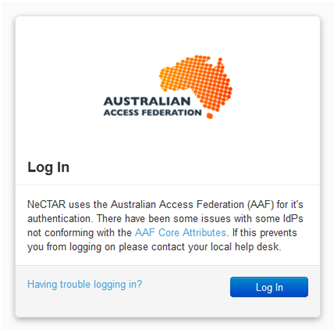
\includegraphics[scale=0.5]{post-workshop/nectar/aaf_login.png}
    \caption{\label{fig:aaf_login}}
  \end{figure}
  \item At the following screen, simply choose your institution from the
  dropdown box and click ``Select". Now follow the on screen prompts and enter
  your regular institutional login details.
  \begin{figure}[H]
    \centering
    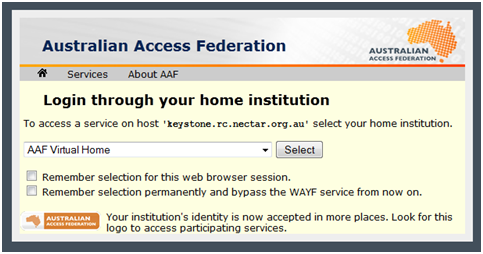
\includegraphics[scale=0.5]{post-workshop/nectar/aaf_home_institute.png}
    \caption{\label{fig:aaf_home_institute}}
  \end{figure}
  \item If you see the following screen, congratulations, you have
  successfully logged into the NeCTAR Research Cloud dashboard!
  \begin{figure}[H]
    \centering
    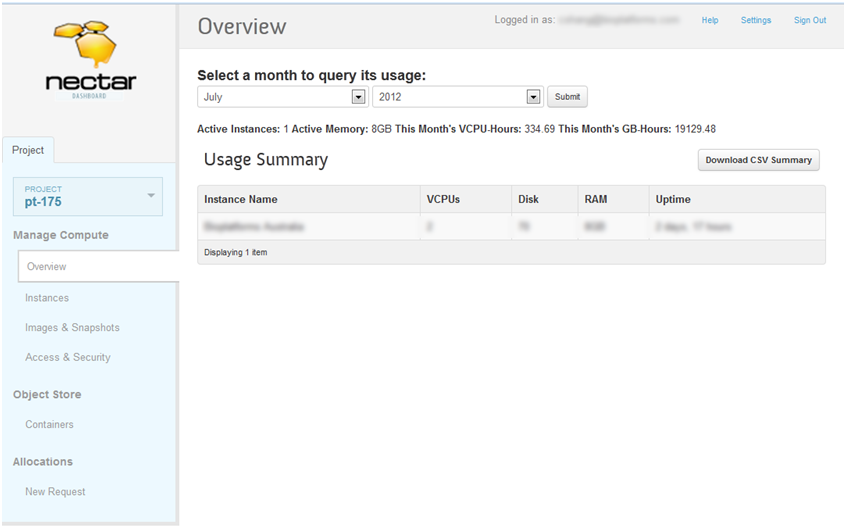
\includegraphics[scale=0.5]{post-workshop/nectar/dashboard_overview.png}
    \caption{\label{fig:dashboard_overview}}
  \end{figure}
\end{enumerate}

\subsubsection{Instantiating Your Own VM}
We will now show you how to instantiate the ``NGS Training'' image using your
own personal cloud allocation.

\begin{enumerate}
  \item In the NeCTAR Research Cloud dashboard, click ``Images \& Snapshots''
  to list all the publicly available images from which you can instantiate a
  VM. Under ``Snapshots" Click the ``Launch" button for the latest version of the
  ``NGSTraining" snapshot:
  \begin{figure}[H]
    \centering
    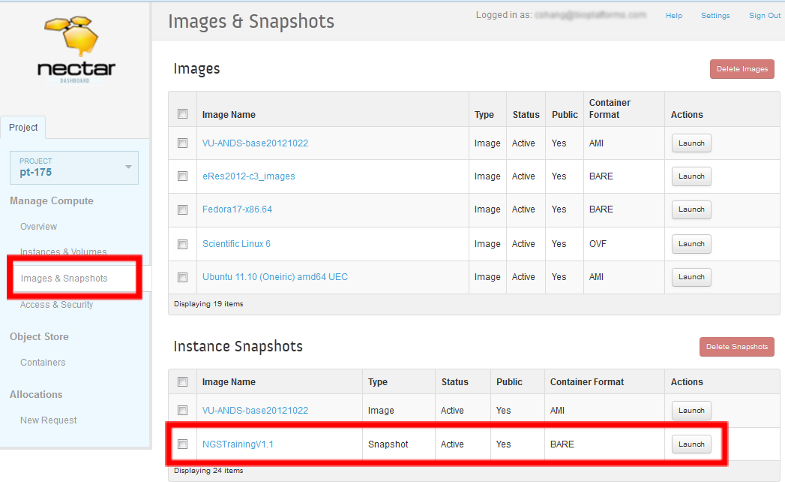
\includegraphics[scale=0.5]{post-workshop/nectar/dashboard_snapshots.png}
    \caption{\label{fig:dashboard_snapshots}}
  \end{figure}
  \item You will now see a ``Launch Instances'' window where you are required to
  enter some details about how you want the VM to be setup before clicking
  ``Launch Instance".
  In the ``Launch Instances'' pop-up frame choose the following settings:
  \begin{description}
  \item[Server Name] A human readable name for your convenience. e.g. ``My NGS VM''
  \item[Flavor] The resources you want to allocate to this VM. I suggest a
  Medium sized VM (2 CPUs and 8 GBytes RAM). This will use all your personal
  allocation, but anything less will probably be insufficient. You could request
  a new allocation of resources if you want to instantiate a larger VM with more
  memory.
  \item[Security Groups] Select SSH.
  \end{description}
  \item Click the ``Launch Instance'' button
  \begin{figure}[H]
    \centering
    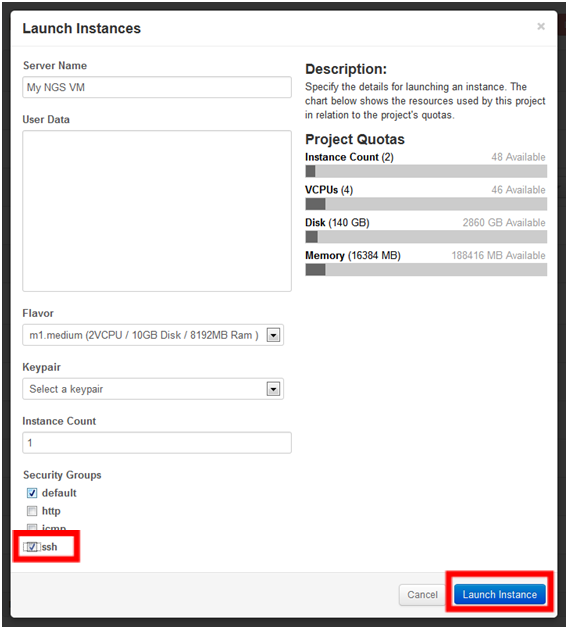
\includegraphics[scale=0.5]{post-workshop/nectar/dashboard_launch.png}
    \caption{\label{fig:dashboard_launch}}
  \end{figure}
  \item You will be taken to the ``Instances" page and you will see the
  ``Status" and ``Task" column for your new VM is ``Building" and ``Spawning". Once
  the ``IP Address" cell is populated, take a note of it as you will need it for
  configuring the NX Client later on.
  \begin{figure}[H]
    \centering
    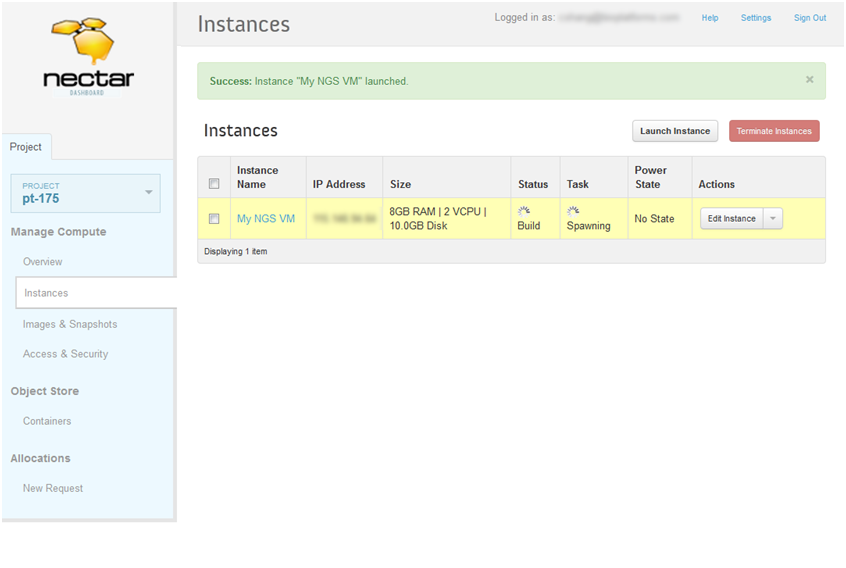
\includegraphics[scale=0.5]{post-workshop/nectar/dashboard_instance_building.png}
    \caption{\label{fig:dashboard_instance_building}}
  \end{figure}
  \item Once the Status and Task for the VM change to ``Active and ``None"
  respectively, your VM is powered up and is configuring itself.
  Congratulations, you have now instantiated a Virtual Machine! If you try to
  connect to the VM too quickly, you might not be successful. The OS may still
  be configuring itself, so give it a few minutes to finish before continuing.
  \begin{figure}[H]
    \centering
    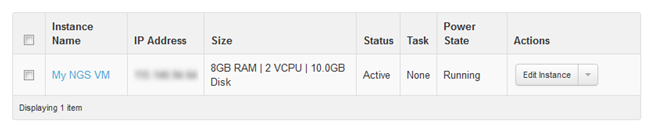
\includegraphics[scale=0.5]{post-workshop/nectar/dashboard_instance_running.png}
    \caption{\label{fig:dashboard_instance_running}}
  \end{figure}
\end{enumerate}

\subsubsection{VM Stuck Building and Spawning}
Sometimes, the cloud experiences a ``hiccup" and a newly instantiated VM will get
stuck in the ``Build" and ``Spawning" state (step 3) for more than a few minutes.
This can be rectified by terminating the instance and creating a new VM from
scratch:
\begin{enumerate}
  \item Selecting ``Terminate Instance" under the ``Edit Instance" dropdown box:
  \begin{figure}[H]
    \centering
    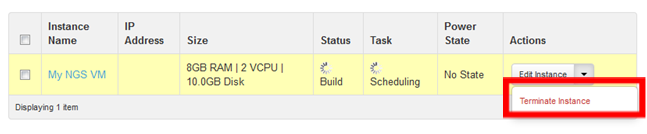
\includegraphics[scale=0.5]{post-workshop/nectar/dashboard_terminate_stuck_instance.png}
    \caption{\label{fig:dashboard_terminate_stuck_instance}}
  \end{figure}
  \item Go back to step 1 of ``Instantiating Your Own VM" and create the VM from scratch:
\end{enumerate}
  

\subsection{Remote Desktop with the NoMachine NX Client}
During the workshop you were using the free NX client from NoMachine
(\url{http://www.nomachine.com/}) to provide a remote desktop-like connection to
VMs running on the NeCTAR Research Cloud. Therefore, we provide information on how to
setup your local computer to connect to the VM you just instantiated in the steps
above.

We assume that:
\begin{itemize}
\item You have administrator rights on your local computer for installing
software.
\end{itemize}

\subsubsection{NoMachine NX Client Installing}
We show you instructions below for the MS Windows version of the NX Client, but
procedures for other supported OSes (Linux, Mac OSX and Solaris) should be very
similar.
\begin{enumerate}
  \item Go to the NoMachine download page: \url{http://www.nomachine.com/download.php}
  \item Click the download icon next to the NX Client for Windows:
  \begin{figure}[H]
    \centering
    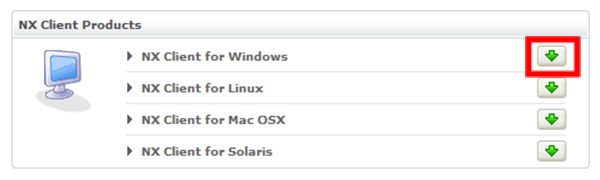
\includegraphics[scale=0.5]{post-workshop/nx_client/download.png}
    \caption{\label{fig:nx_download}}
  \end{figure}
  \item On the "NX Client for Windows" page, click the "Download package" button:
  \begin{figure}[H]
    \centering
    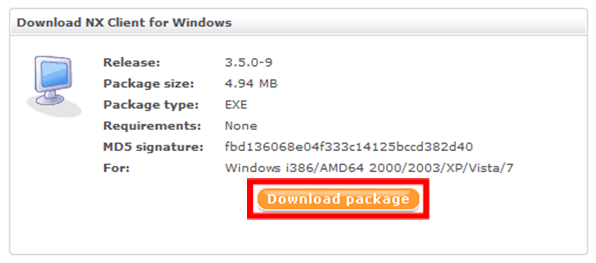
\includegraphics[scale=0.5]{post-workshop/nx_client/download_package.png}
    \caption{\label{fig:nx_download_package}}
  \end{figure}
  \item Run the file you just downloaded (accepting defaults is fine)
  \item Congratulations, you just installed the NoMachine NX Client!
\end{enumerate}

\subsection{NoMachine NX Client Configuration}
Now we have the NoMachine NX Client installed, we need to configure a new NX
"session" which will point to the VM we instantiated in the NeCTAR Research
Cloud.

We assume that:
\begin{itemize}
\item You know the IP address of the VM you want to remote desktop into.
\end{itemize}

\begin{enumerate}
  \item Start the NX Connection Wizard and click "Next" to advance to the
  "Session" settings page.
  \begin{figure}[H]
    \centering
    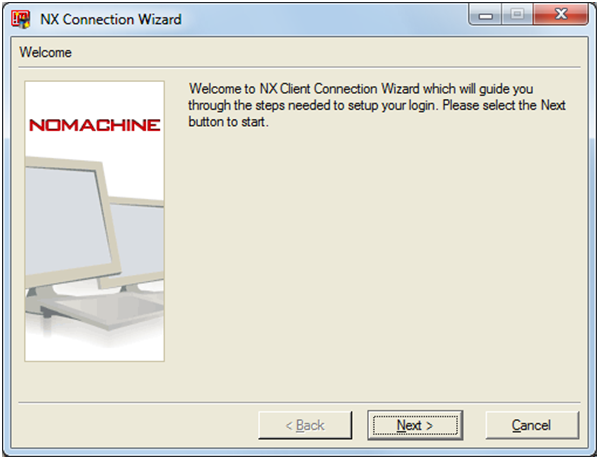
\includegraphics[scale=0.5]{post-workshop/nx_client/start_wizard.png}
    \caption{\label{fig:nx_start_wizard}}
  \end{figure}
  \item On the "Sessions" settings page enter the following details:
  \begin{description}
  \item[Session] A memorable name so you know which VM this session is pointing
  at. You could use the same name you chose for the VM you instantiated earlier
  e.g. "NGS Training".
  \item[Host] Enter the IP address of the VM you instantiated on the NeCTAR
  Research Cloud.
  \begin{figure}[H]
    \centering
    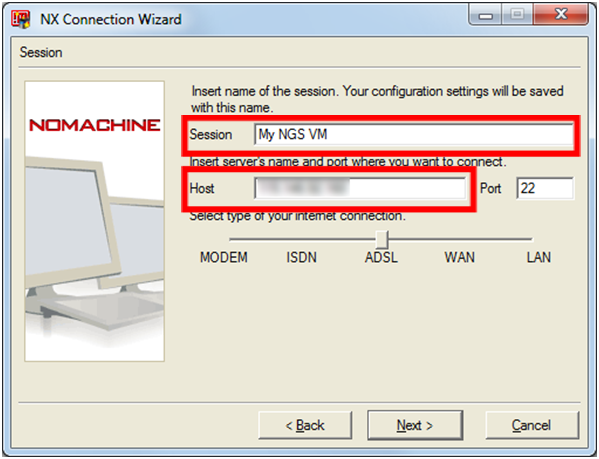
\includegraphics[scale=0.5]{post-workshop/nx_client/session_configuration.png}
    \caption{\label{fig:nx_session_configuration}}
  \end{figure}
  \end{description}
  \item Click "Next" to advance to the "Desktop" settings page. You should use the
  "Unix GNOME" setting.
  \begin{figure}[H]
    \centering
    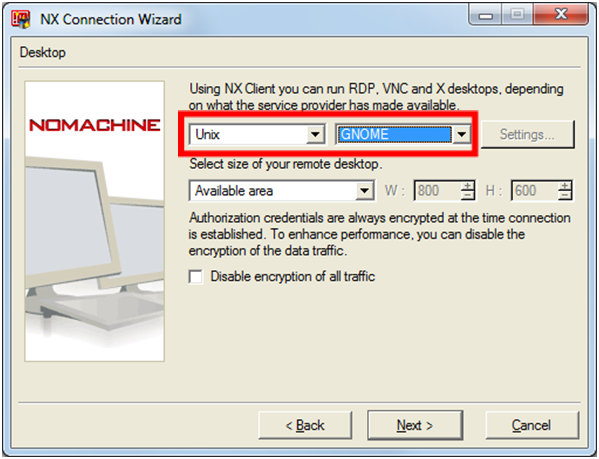
\includegraphics[scale=0.5]{post-workshop/nx_client/desktop_type.png}
    \caption{\label{fig:nx_desktop_type}}
  \end{figure}
  \item Click "Next" and "Finish" to complete the wizard.
\end{enumerate}

\subsection{Connecting to a VM}
If you just completed the NX Connection Wizard described above, the wizard
should have opened the NX Client window. If not, run the "NX Client". You will
be presented with a window like this:
\begin{figure}[H]
  \centering
  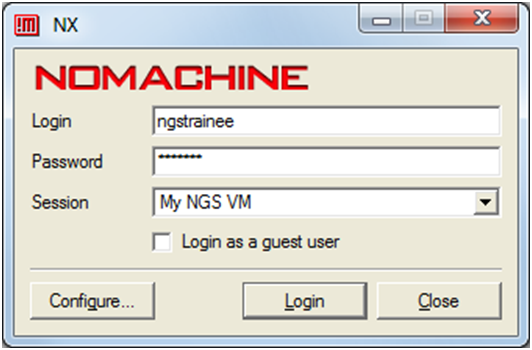
\includegraphics[scale=0.5]{post-workshop/nx_client/login.png}
  \caption{\label{fig:nx_login}}
\end{figure}

The "Login" and "Password" boxes in the NX Client are for user accounts setup on
the VM. By default our image, from which you instantiated your VM, has two
preconfigured users:
\begin{figure}[H]
  \centering
  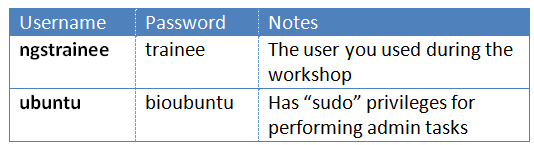
\includegraphics[scale=0.5]{post-workshop/nx_client/usernames_passwords.png}
  \caption{\label{fig:nx_usernames_passwords}}
\end{figure}

Unless you know what you are doing, we suggest you use the \texttt{ngstrainee}
user account details to initiate an NX connection to your VM. In less than a
minute, you should see an NX Window showing the desktop of your VM:
\begin{figure}[H]
  \centering
  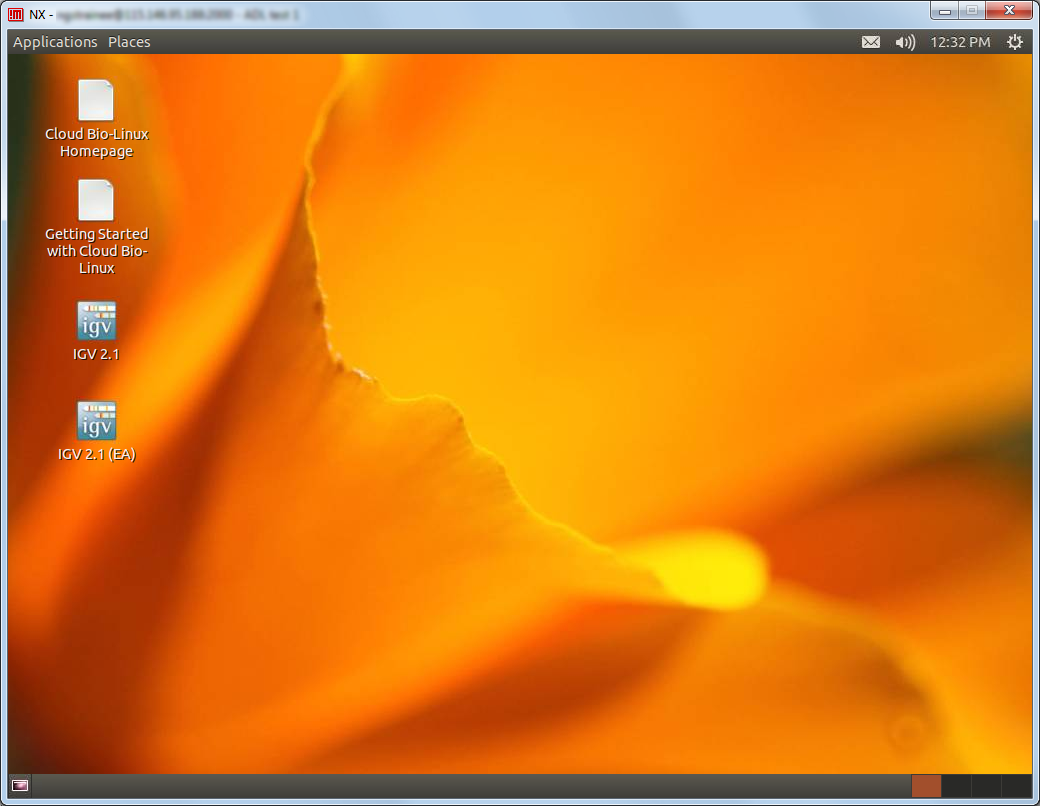
\includegraphics[width=0.8\textwidth]{post-workshop/nx_client/connected.png}
  \caption{\label{fig:nx_connected}}
\end{figure}

\subsection{NX Connection Failure}
In the event that you don't get the NX Window with your VM's desktop displaying
inside it. The most common errors are:
\begin{itemize}
\item You failed to select the "ssh" security group when instantiating the VM.
You'll need to terminate the instance and create a new VM from scratch
\item You failed to select "Unix GNOME" when you configured the NX Client
session. You'll need to reconfigure the session using the NX Client
\item Your institutions firewall blocks TCP port 22. You may need to request this
port to be opened by your local network team or configure the NX client to use a
proxy server.
\end{itemize}

\subsection{Advanced Configuration}
In the session configuration, you can configure the size of the NX Window in
which the desktop of the VM is drawn:
\begin{figure}[H]
  \centering
  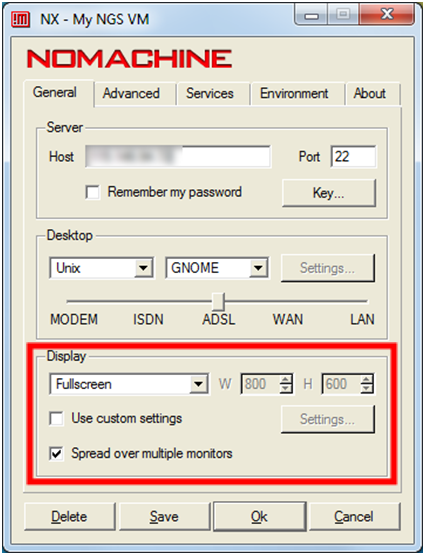
\includegraphics[scale=0.5]{post-workshop/nx_client/advanced_display.png}
  \caption{\label{fig:nx_advanced_display}}
\end{figure}

This can be useful if you want to:
\begin{itemize}
\item Have the NX Window occupy the entire screen, without window decorations.
This is often desirable if you wish to "hide" the host OS from the person
sitting at the computer running the NX Client.
\item Have the NX Window spread over multiple monitors.
\end{itemize}


\clearpage

%
% Access to Workshop Documents
%
\section{Access to Workshop Documents}

This document has been written in \LaTeX\ and deposited in a public github
repository (\url{https://github.com/nathanhaigh/ngs_workshop}). The
documentation has been released under a Creative Commons Attribution 3.0
Unported License (see the Licence page at the beginning of this handout).

For convienience, you can access up-to-date PDF versions of the \LaTeX\ documents at:
\begin{description}[style=multiline,labelindent=0cm,align=left,leftmargin=0.5cm]
\item[Trainee Handout]\hfill\\
\url{https://github.com/downloads/nathanhaigh/ngs_workshop/trainee_handout_latest.pdf}
\item[Trainer Handout]\hfill\\
\url{https://github.com/downloads/nathanhaigh/ngs_workshop/trainer_handout_latest.pdf}
\end{description}

\section{Access to Workshop Data}
Once you have created a VM from our image file, either locally using VirtualBox
or on the NeCTAR Research Cloud, you can configure the system with the workshop
documents and data. This way you can revisit and work through this workshop in
your own time.

In order to do this, we have provided you with access to a shell script which
should be executed on your NGS Training VM by the \texttt{ubuntu} user. This pulls
approx. 3.3 GBytes of data from the NeCTAR Cloud storage and configures the system
for running this workshop:

% NOTE This bash script could be entered into the user data when instantiating
% the VM in the first place
\begin{lstlisting}
# As the ubuntu user run the following commands:
cd /tmp
wget https://github.com/nathanhaigh/ngs_workshop/raw/master/\
workshop_setup/setup_NGS_workshop.sh
bash setup_NGS_workshop.sh
\end{lstlisting}

While you're at it, you may also like to change the timezone of your VM to match
that of your own. To do this simply run the following commands as the
\texttt{ubuntu} user:
\begin{lstlisting}
TZ="Australia/Adelaide"
echo "$TZ" | sudo tee /etc/timezone
sudo dpkg-reconfigure --frontend noninteractive tzdata
\end{lstlisting}

For further information about what this script does and possible command line
arguments, see the script's help:
\begin{lstlisting}
bash setup_NGS_workshop.sh -h
\end{lstlisting}


For further information about setting up the VM for the workshop, please see:
\\\\
\url{https://github.com/nathanhaigh/ngs_workshop/blob/master/workshop_setup/README.md}


\chapter{Space for Personal Notes or Feedback}
\clearpage

%
% Some empty ruled comments pages
%
\myruledpage{3cm}{1cm}
\myruledpage{3cm}{1cm}
\myruledpage{3cm}{1cm}
\myruledpage{3cm}{1cm}

\end{document}
